\section{Seitenersetzungsstrategien}\label{Seiten}
Für einen Puffer stehen drei Kacheln im Hauptspeicher zur Verfügung. Es soll nun bestimmt werden, wie sich eine Seitenersetzungsstrategie bei einem bestimmten Zugriffsmuster auf Seiten verhält.

\begin{enumerate}[a)]
    \item Diskutieren Sie die Funktionsweise und Eignung der Strategien LFU und LRU.
\begin{solution}
    \begin{itemize}
        \item \textbf{LFU} (Least Frequently Used):
					Block, auf den am seltensten zugegriffen wurde, wird ersetzt. (Bei Gleichstand in der Benutzungshäufigkeit kann beispielsweise die Seite verdrängt werden, die länger im Hauptspeicher ist.)

            Eignung von LFU: Die Häufigkeit der Nutzung eines Blocks sagt nicht unbedingt etwas über die Häufigkeit der Nutzung in Zukunft aus.
            Werden beispielsweise kurzfristig sehr viele Daten aus einem Block benötigt, z.B. aus einem Index, hält sich dieser anschließend so lange, bis ein weiterer Block ebenfalls so häufig genutzt wurde.
            Im Beispiel wird dann der Index über lange Zeit im Puffer gehalten, obwohl er vielleicht längst nicht mehr benötigt würde und der Platz viel sinnvoller für Blöcke mit Anwendungsdaten genutzt werden könnte.

        \item \textbf{LRU} (Least Recently Used):
            Block, auf den am längsten nicht zugegriffen wurde, wird ersetzt.

            Eignung von LRU: LRU berücksichtigt sowohl das Alter als auch die Benutzungshäufigkeit, so dass die bei LFU (bzw. FIFO) auftretenden Probleme gelöst sind. Allerdings ist die Ermittlung der zu verdrängenden Seite bei LRU und LFU im Gegensatz zu z.B. FIFO aufwändiger.
    \end{itemize}

\end{solution}
\beamertxt{\pagebreak}

	\item
Modellieren Sie die folgende Referenzfolge mit der Seitenersetzungsstrategie CLOCK. Beurteilen Sie auch, wie gut die vorgegebene Strategie zur Referenzfolge passt und wo die Strategie ungünstige Entscheidungen trifft.

Zu Beginn seien alle Kacheln leer. Geben Sie an, welche Seiten zu welchen Zeitpunkten in den Kacheln des Prozesses eingelagert sind. Notieren Sie auch die Kontrollzustände für jede Belegung. Im Falle von CLOCK ist das das Benutzt-Bit. Geben Sie außerdem die Anzahl der Seitenfehler an, d.\,h. die Anzahl der Seiten, die vom Hintergrundspeicher geladen werden müssen. Die Einlagerungen der ersten drei Seiten sollen auch als Seitenfehler mitgezählt werden.

Reihenfolge der Seitenreferenzen: $1, 2, 3, 5, 1, 1, 4, 1, 2, 1, 3, 1$.

\begin{beamerText}
\begin{samepage}
\begin{Form}
\begin{center}
	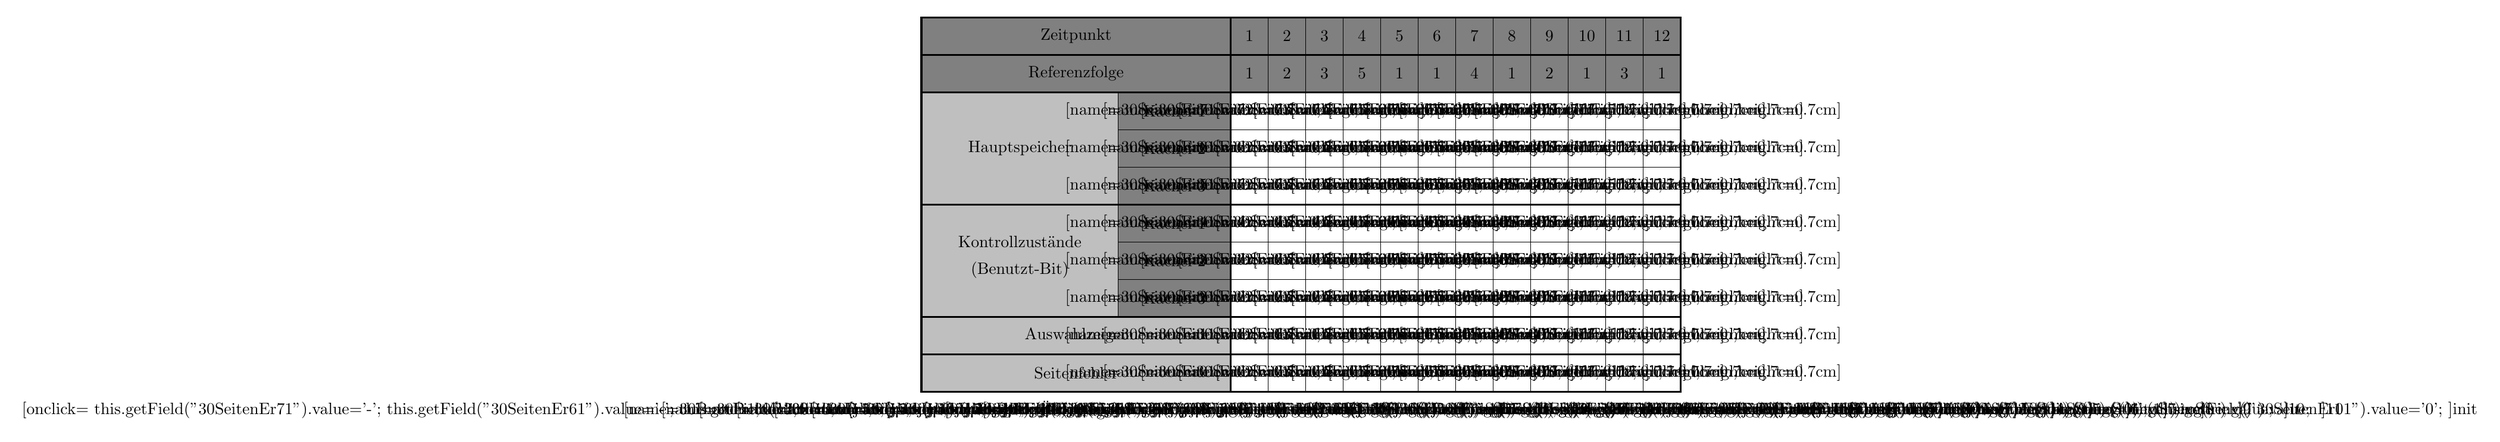
\begin{tikzpicture}
		\fill[fill=lightgray]
			(-1, 0.8) rectangle+(4.2, 4.8)
			(-1, -0.8) rectangle+(6.6, 1.6);
		\fill[fill=gray]
			(3.2, 0.8) rectangle+(2.4, 4.8)
			(-1, 5.6) rectangle+(16.2, 1.6);

		\draw (3.2, 4.8) -- (5.6, 4.8);
		\draw (3.2, 4) -- (5.6, 4);
		\draw (3.2, 2.4) -- (5.6, 2.4);
		\draw (3.2, 1.6) -- (5.6, 1.6);
		\draw (3.2, 0.8) -- (3.2, 5.6);
		\draw[step =.8cm] (5.6, -0.8) grid+(9.6, 8);
		\draw[very thick] (-1, -0.8) rectangle+(16.2, 8);
		\draw[very thick] (-1, 3.2) -- (15.2, 3.2);
		\draw[very thick] (-1, 0.8) -- (15.2, 0.8);
		\draw[very thick] (-1, 0) -- (15.2, 0);
		\draw[very thick] (-1, 6.4) -- (15.2, 6.4);
		\draw[very thick] (-1, 5.6) -- (15.2,5.6);
		\draw[very thick] (5.6, -0.8) -- (5.6, 7.2);

		\node at (2.3, 6.8) {Zeitpunkt};
		\node at (2.3, 6) {Referenzfolge};
		\node[text=black] at (1.1, 4.4) {Hauptspeicher};
		\node[text=black] at (1.1, 2.4) {Kontrollzustände};
		\node[text=black] at (1.1, 1.8) {(Benutzt-Bit)};
		\node at (4.4, 5.2) {Kachel 1};
		\node at (4.4, 4.4) {Kachel 2};
		\node at (4.4, 3.6) {Kachel 3};
		\node at (4.4, 2.8) {Kachel 1};
		\node at (4.4, 2) {Kachel 2};
		\node at (4.4, 1.2) {Kachel 3};
		\node[text=black] at (2.3, 0.4) {Auswahlzeiger};
		\node[text=black] at (2.3, -0.4) {Seitenfehler};
		\node at (2.3, -1.2) {Übertrage};
		%pageref
		\node at(6, 6.8) {1};
		\node at(6.8, 6.8) {2};
		\node at(7.6, 6.8) {3};
		\node at(8.4, 6.8) {4};
		\node at(9.2, 6.8) {5};
		\node at(10, 6.8) {6};
		\node at(10.8, 6.8) {7};
		\node at(11.6, 6.8) {8};
		\node at(12.4, 6.8) {9};
		\node at(13.2, 6.8) {10};
		\node at(14, 6.8) {11};
		\node at(14.8, 6.8) {12};
		%ref
		\node at(6, 6) {1};
		\node at(6.8, 6) {2};
		\node at(7.6, 6) {3};
		\node at(8.4, 6) {5};
		\node at(9.2, 6) {1};
		\node at(10, 6) {1};
		\node at(10.8, 6) {4};
		\node at(11.6, 6) {1};
		\node at(12.4, 6) {2};
		\node at(13.2, 6) {1};
		\node at(14, 6) {3};
		\node at(14.8, 6) {1};
		%HK1
		\foreach \j in {0,...,7}
		\foreach \i in {1,...,12}
		{
			\node at (5.105+0.8*\i, -0.4 + 0.8*\j) {\TextField[name=30SeitenEr\j\i,width=0.7cm,height=0.7cm]{\null}};
		}

		\node at (6.005, -1.2) {\PushButton[onclick={
				this.getField("30SeitenEr71").value='-';
				this.getField("30SeitenEr61").value='-';
				this.getField("30SeitenEr51").value='-';
				this.getField("30SeitenEr41").value='0';
				this.getField("30SeitenEr31").value='0';
				this.getField("30SeitenEr21").value='0';
				this.getField("30SeitenEr11").value='1';
				this.getField("30SeitenEr01").value='0';
			}]{init}};

		\foreach \i in{1,...,11}
		{
			\node at (6.005+0.8*\i, -1.2) {\PushButton[name=30Button\i,onclick={
			for(j=0; j<8; j++){
				this.getField(
					"30SeitenEr"+j.toString() + (\i+1).toString()
				).value=this.getField(
					"30SeitenEr"+j.toString() + (\i).toString()
				).value;
			}
			}]{\i}};
		}
	\end{tikzpicture}
\PushButton[onclick={
for(i=1; i< 13; i++) {
for(j=0; j<8; j++){
	this.getField("30SeitenEr" + j.toString() + i.toString()).value='';
}
}
}]{Clear}
\end{center}
\end{Form}
\end{samepage}
\end{beamerText}

\begin{normalText}

\begin{center}
	\begin{tikzpicture}
		\fill[fill=lightgray]
			(0, 0) rectangle+(3.2, 5.6)
			(3.2, 0) rectangle+(2.4, 0.8);
		\fill[fill=gray]
			(3.2, 0.8) rectangle+(2.4, 4.8)
			(0, 5.6) rectangle+(15.2, 1.6);

		\draw (3.2, 4.8) -- (5.6, 4.8);
		\draw (3.2, 4) -- (5.6, 4);
		\draw (3.2, 2.4) -- (5.6, 2.4);
		\draw (3.2, 1.6) -- (5.6, 1.6);
		\draw (3.2, 0.8) -- (3.2, 5.6);
		\draw[step =.8cm] (5.6, 0) grid+(9.6, 7.2);
		\draw[very thick] (0, 0) rectangle+(15.2, 7.2);
		\draw[very thick] (0, 3.2) -- (15.2, 3.2);
		\draw[very thick] (0, 0.8) -- (15.2, 0.8);
		\draw[very thick] (0, 6.4) -- (15.2, 6.4);
		\draw[very thick] (0, 5.6) -- (15.2,5.6);
		\draw[very thick] (5.6, 0) -- (5.6, 7.2);

		\node at (2.8, 6.8) {Zeitpunkt};
		\node at (2.8, 6) {Referenzfolge};
		\node at (1.6, 4.4) {Hauptspeicher};
		\node at (1.6, 2.4) {Kontrollzustände};
		\node at (1.6, 1.8) {(Benutzt-Bit)};
		\node at (4.4, 5.2) {Kachel 1};
		\node at (4.4, 4.4) {Kachel 2};
		\node at (4.4, 3.6) {Kachel 3};
		\node at (4.4, 2.8) {Kachel 1};
		\node at (4.4, 2) {Kachel 2};
		\node at (4.4, 1.2) {Kachel 3};
		\node at (2.8, 0.4) {Auswahlzeiger auf Kachel-Nr:};
		%pageref
		\node at(6, 6.8) {1};
		\node at(6.8, 6.8) {2};
		\node at(7.6, 6.8) {3};
		\node at(8.4, 6.8) {4};
		\node at(9.2, 6.8) {5};
		\node at(10, 6.8) {6};
		\node at(10.8, 6.8) {7};
		\node at(11.6, 6.8) {8};
		\node at(12.4, 6.8) {9};
		\node at(13.2, 6.8) {10};
		\node at(14, 6.8) {11};
		\node at(14.8, 6.8) {12};
		%ref
		\node at(6, 6) {1};
		\node at(6.8, 6) {2};
		\node at(7.6, 6) {3};
		\node at(8.4, 6) {5};
		\node at(9.2, 6) {1};
		\node at(10, 6) {1};
		\node at(10.8, 6) {4};
		\node at(11.6, 6) {1};
		\node at(12.4, 6) {2};
		\node at(13.2, 6) {1};
		\node at(14, 6) {3};
		\node at(14.8, 6) {1};
		%HK1
		\node at(6, 5.2) {1};
		\sol[{
			\node[shape=ellipse callout, callout relative pointer={(-2.1cm,0.5cm)},draw, fill=white] at (10,4) {In Kachel 1 ist jetzt Seite 1 eingelagert};
		}]{
			\node at(6.8, 5.2) {1};
			\node at(7.6, 5.2) {1};
			\node at(8.4, 5.2) {5};
			\node at(9.2, 5.2) {5};
			\node at(10, 5.2) {5};
			\node at(10.8, 5.2) {5};
			\node at(11.6, 5.2) {5};
			\node at(12.4, 5.2) {2};
			\node at(13.2, 5.2) {2};
			\node at(14, 5.2) {2};
			\node at(14.8, 5.2) {2};
			%HK2
			\node at(6.8, 4.4) {2};
			\node at(7.6, 4.4) {2};
			\node at(8.4, 4.4) {2};
			\node at(9.2, 4.4) {1};
			\node at(10, 4.4) {1};
			\node at(10.8, 4.4) {1};
			\node at(11.6, 4.4) {1};
			\node at(12.4, 4.4) {1};
			\node at(13.2, 4.4) {1};
			\node at(14, 4.4) {1};
			\node at(14.8, 4.4) {1};
			%HK3
			\node at(7.6, 3.6) {3};
			\node at(8.4, 3.6) {3};
			\node at(9.2, 3.6) {3};
			\node at(10, 3.6) {3};
			\node at(10.8, 3.6) {4};
			\node at(11.6, 3.6) {4};
			\node at(12.4, 3.6) {4};
			\node at(13.2, 3.6) {4};
			\node at(14, 3.6) {3};
			\node at(14.8, 3.6) {3};
			%ctrlK1
		}
		\node at(6, 2.8) {1};
		\sol[{
			\node[shape=ellipse callout, callout relative pointer={(-1.7cm,0.5cm)},draw, fill=white] at (10,1.5) {\parbox{5cm}{Benutzt Bit der Kachel 1 wird auf 1 gesetzt}};
		}]{
			\node at(6.8, 2.8) {1};
			\node at(7.6, 2.8) {1};
			\node at(8.4, 2.8) {1};
			\node at(9.2, 2.8) {1};
			\node at(10, 2.8) {1};
			\node at(10.8, 2.8) {1};
			\node at(11.6, 2.8) {1};
			\node at(12.4, 2.8) {1};
			\node at(13.2, 2.8) {1};
			\node at(14, 2.8) {1};
			\node at(14.8, 2.8) {1};
			%ctrlK2
			\node at(6, 2) {0};
			\node at(6.8, 2) {1};
			\node at(7.6, 2) {1};
			\node at(8.4, 2) {0};
			\node at(9.2, 2) {1};
			\node at(10, 2) {1};
			\node at(10.8, 2) {1};
			\node at(11.6, 2) {1};
			\node at(12.4, 2) {0};
			\node at(13.2, 2) {1};
			\node at(14, 2) {0};
			\node at(14.8, 2) {1};
			%ctrlK3
			\node at(6, 1.2) {0};
			\node at(6.8, 1.2) {0};
			\node at(7.6, 1.2) {1};
			\node at(8.4, 1.2) {0};
			\node at(9.2, 1.2) {0};
			\node at(10, 1.2) {0};
			\node at(10.8, 1.2) {1};
			\node at(11.6, 1.2) {1};
			\node at(12.4, 1.2) {0};
			\node at(13.2, 1.2) {0};
			\node at(14, 1.2) {1};
			\node at(14.8, 1.2) {1};
		}
		%pointer
		\node at(6, 0.4) {2};
		\sol{
			\node at(6.8, 0.4) {3};
			\node at(7.6, 0.4) {1};
			\node at(8.4, 0.4) {2};
			\node at(9.2, 0.4) {3};
			\node at(10, 0.4) {3};
			\node at(10.8, 0.4) {1};
			\node at(11.6, 0.4) {1};
			\node at(12.4, 0.4) {2};
			\node at(13.2, 0.4) {2};
			\node at(14, 0.4) {1};
			\node at(14.8, 0.4) {1};
		}
	\end{tikzpicture}
	\end{center}
\end{normalText}
\begin{solution}[Anzahl Seitenfehler: bisher 1 (Einlagern von Seite 1)]
	Anzahl Seitenfehler: bei Seitenreferenz 1, 2, 3, 5, 1, 4, 2, 3 also insgesamt 8

	Der Auswahlzeiger zeigt stets auf die Kachel, die für das Ersetzen als nächstes geprüft wird (sowohl wenn eine Seite eingefügt wurde, als auch wenn eine Seite schon im Puffer war und das Benutzt-Bit wieder auf 1 gesetzt wurde).

	Eignung von CLOCK: Ressourcenschonend, da lediglich ein Bit „Verwaltungsstruktur“ für jeden Puffer dazukommt, bzw. eine externe Bitmap mit der Anzahl der verwalteten Pufferblöcke geführt und durchsucht wird. CLOCK berücksichtigt jedoch nicht die Anzahl der Zugriffe. Jede Seite überlebt mindestens zwei „Zeigerumläufe“. Kann zu FIFO degenerieren, wenn alle Benutzt-Bits 1 sind (siehe Aufgabe).
	\subsection*{Ersetzungsverfahren und Lokalität}
\begin{minipage}{0.45\textwidth}
	Grundannahme bei Ersetzungsverfahren ist: Das Referenzverhalten der jüngsten Vergangenheit ist ähnlich dem der nächsten Zukunft $\rightarrow$ typischerweise hat man hohe Lokalität (d.h. in einem bestimmten Zeitintervall wird auf einem relativ kleinen Bereich Datenmenge gearbeitet). Hat man dagegen nur zufällige Zugriffe braucht man auch nicht Puffern -- bringt nichts, kostet nur ($\rightarrow$ Thrashing).
\end{minipage}
\begin{minipage}{0.5\textwidth}
	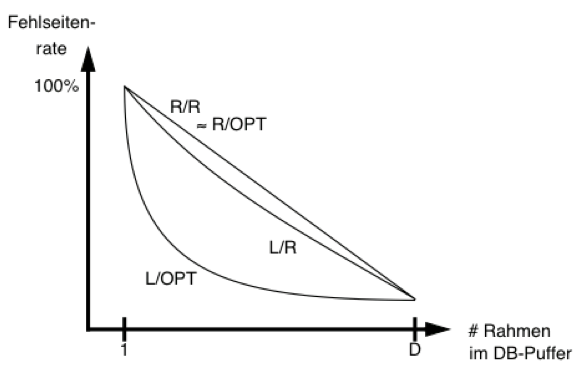
\includegraphics[width = 8cm]{Pictures/Ue07_Aufgabe2_Zusatz1.png}
\end{minipage}

\begin{tabular}{|l|l|l|l|l|}
	\hline
	 					& R/R 			& R/OPT 		& L/R 			& L/OPT 		\\
	\hline
	Referenzen 	& Random 	& Random 	& Lokalität 	& Lokalität 	\\
	\hline
	Ersetzung 	& Random 	& Opt 			& Random 	& Opt 			\\
	\hline
\end{tabular}

Belady-Optimal: Ersetze die Seite, die am längsten in die Zukunft nicht referenziert wird.
\end{solution}

\begin{beamerText}
\pagebreak
\subsection*{Ersetzungsverfahren und Lokalität}
\begin{minipage}{0.45\textwidth}
	Grundannahme bei Ersetzungsverfahren ist: Das Referenzverhalten der jüngsten Vergangenheit ist ähnlich dem der nächsten Zukunft $\rightarrow$ typischerweise hat man hohe Lokalität (d.h. in einem bestimmten Zeitintervall wird auf einem relativ kleinen Bereich Datenmenge gearbeitet). Hat man dagegen nur zufällige Zugriffe braucht man auch nicht Puffern -- bringt nichts, kostet nur ($\rightarrow$ Thrashing).
\end{minipage}
\begin{minipage}{0.5\textwidth}
	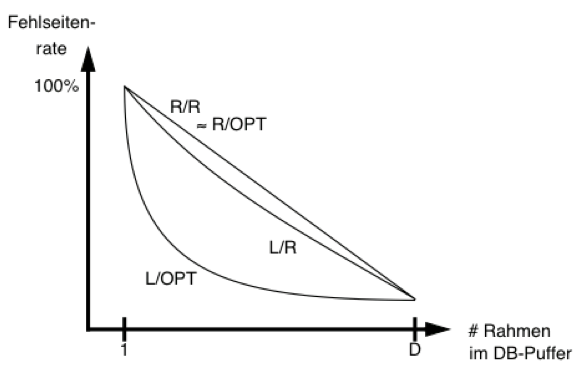
\includegraphics[width = 8cm]{Pictures/Ue07_Aufgabe2_Zusatz1.png}
\end{minipage}

\begin{tabular}{|l|l|l|l|l|}
	\hline
	 					& R/R 			& R/OPT 		& L/R 			& L/OPT 		\\
	\hline
	Referenzen 	& Random 	& Random 	& Lokalität 	& Lokalität 	\\
	\hline
	Ersetzung 	& Random 	& Opt 			& Random 	& Opt 			\\
	\hline
\end{tabular}

Belady-Optimal: Ersetze die Seite, die am längsten in die Zukunft nicht referenziert wird.
\pagebreak
\end{beamerText}

\item Gegeben ist die folgende Seitenreferenzfolge für die Zeitpunkte \(t=1\) bis \(t=13\):
\(1, 2, 1, 3, 1, 2, 1, 2, 3, 4, 5, 6, 7\)

Bestimmen Sie die Working Set Size und die aktuelle Lokalität für eine Fenstergröße von \(w = 8\) für die Zeitpunkte \(t=8\) und \(t=13\).
Bestimmen Sie weiterhin die durchschnittliche Lokalität für diese Fenstergröße und die gegebene Referenzfolge.

\begin{solution}
Die Anzahl an unterschiedlichen referenzierten Seiten bei $w$ Zugriffen nennen wir Working Set Size. Betrachten wir  die ersten 8 (\(t=8\)) und die letzten 8 Zugriffe (\(t=13\)), dann sehen wir, dass im ersten Fall 3 unterschiedliche Werte auftreten und im anderen Fall 7 $\rightarrow$ die Working Set Size $|W|$ beträgt im ersten Fall also $3$ und im zweiten Fall $7$.

Die aktuelle Lokalität ist dann gegeben durch	\[AL(t, w) = \frac{|W(t, w)|}{w}\] d.\,h. $\frac{3}{8}$
für \(t=8\), und $\frac{7}{8}$ für \(t=13\).

Die durchschnittliche Lokalität ist: \[L(w) = \frac{\sum_{t = w}^n AL(t, w)}{n-(w-1)}\]
Für die gegebene Referenzfolge ergibt sich eine durchschnittliche Lokalität von:
\begin{equation*}
	 L(8) = \frac{\sum_{t = 8}^{13} AL(t, 8)}{6} = \frac{1}{6} \cdot (\frac{3}{8}+\frac{3}{8}+\frac{4}{8}+\frac{5}{8}+\frac{6}{8}+\frac{7}{8}) = \frac{7}{12}
\end{equation*}

\end{solution}

    \item Bestimmen Sie für die Seitenreferenzfolge $1, 2, 3, 5, 1, 1, 4, 1, 2, 1, 3, 1$ die LRU-Stack\-tie\-fen\-ver\-tei\-lung.

\begin{solution}
Der LRU-Stack enthält alle bereits referenzierten Seiten in der Reihenfolge ihres Zugriffsalters. Wie bestimmt man die Stacktiefen-Verteilung? Pro Stackposition gibt es einen Zähler; Referenz einer Seite führt zu Zählererhöhung an der jew. Stackposition ($\rightarrow$ Zählerwerte entsprechen Wiederbenutzungshäufigkeit)


    \begin{minipage}{0.28\textwidth}
        \center
        Zugriff auf 1, 2, 3, 5:

        \begin{tabular}{ | c | l}
            \cline{1-1}
            5   &   0   \\  \cline{1-1}
            3   &   0   \\  \cline{1-1}
            2   &   0   \\  \cline{1-1}
            1   &   0   \\  \cline{1-1}
                &   0   \\  \cline{1-1}
                &   0   \\  \cline{1-1}
        \end{tabular}
    \end{minipage}
    \begin{minipage}{0.22\textwidth}
        \center
        Zugriff auf 1:

        \begin{tabular}{ | c | l}
            \cline{1-1}
            1   &   0   \\  \cline{1-1}
            5   &   0   \\  \cline{1-1}
            3   &   0   \\  \cline{1-1}
            2   &   1   \\  \cline{1-1}
                &   0   \\  \cline{1-1}
                &   0   \\  \cline{1-1}
        \end{tabular}
    \end{minipage}
    \begin{minipage}{0.22\textwidth}
        \center
        Zugriff auf 1:

        \begin{tabular}{ | c | l}
            \cline{1-1}
            1   &   1   \\  \cline{1-1}
            5   &   0   \\  \cline{1-1}
            3   &   0   \\  \cline{1-1}
            2   &   1   \\  \cline{1-1}
                &   0   \\  \cline{1-1}
                &   0   \\  \cline{1-1}
        \end{tabular}
    \end{minipage}
    \begin{minipage}{0.22\textwidth}
        \center
        Zugriff auf 4:

        \begin{tabular}{ | c | l}
            \cline{1-1}
            4   &   1   \\  \cline{1-1}
            1   &   0   \\  \cline{1-1}
            5   &   0   \\  \cline{1-1}
            3   &   1   \\  \cline{1-1}
            2   &   0   \\  \cline{1-1}
                &   0   \\  \cline{1-1}
        \end{tabular}
    \end{minipage}

    \begin{minipage}{0.28\textwidth}
        \center
        Zugriff auf 1:

        \begin{tabular}{ | c | l}
            \cline{1-1}
            1   &   1   \\  \cline{1-1}
            4   &   1   \\  \cline{1-1}
            5   &   0   \\  \cline{1-1}
            3   &   1   \\  \cline{1-1}
            2   &   0   \\  \cline{1-1}
                &   0   \\  \cline{1-1}
        \end{tabular}
    \end{minipage}
    \begin{minipage}{0.22\textwidth}
        \center
        Zugriff auf 2:

        \begin{tabular}{ | c | l}
            \cline{1-1}
            2   &   1   \\  \cline{1-1}
            1   &   1   \\  \cline{1-1}
            4   &   0   \\  \cline{1-1}
            5   &   1   \\  \cline{1-1}
            3   &   1   \\  \cline{1-1}
                &   0   \\  \cline{1-1}
        \end{tabular}
    \end{minipage}
    \begin{minipage}{0.22\textwidth}
        \center
        Zugriff auf 1:

        \begin{tabular}{ | c | l}
            \cline{1-1}
            1   &   1   \\  \cline{1-1}
            2   &   2   \\  \cline{1-1}
            4   &   0   \\  \cline{1-1}
            5   &   1   \\  \cline{1-1}
            3   &   1   \\  \cline{1-1}
                &   0   \\  \cline{1-1}
        \end{tabular}
    \end{minipage}
    \begin{minipage}{0.22\textwidth}
        \center
        Zugriff auf 3:

        \begin{tabular}{ | c | l}
            \cline{1-1}
            3   &   1   \\  \cline{1-1}
            1   &   2   \\  \cline{1-1}
            2   &   0   \\  \cline{1-1}
            4   &   1   \\  \cline{1-1}
            5   &   2   \\  \cline{1-1}
                &   0   \\  \cline{1-1}
        \end{tabular}
    \end{minipage}

        \begin{minipage}{0.28\textwidth}
            \center
            Zugriff auf 1:

            \begin{tabular}{ | c | l}
                \cline{1-1}
                1   &   1   \\  \cline{1-1}
                3   &   3   \\  \cline{1-1}
                2   &   0   \\  \cline{1-1}
                4   &   1   \\  \cline{1-1}
                5   &   2   \\  \cline{1-1}
                    &   0   \\  \cline{1-1}
            \end{tabular}
        \end{minipage}
        \begin{minipage}{0.65\textwidth}
            Endergebnis (von oberster zu niedrigster Stackposition):

						1, 3, 0, 1, 2
        \end{minipage}

\end{solution}

\item Welche Informationen liefert die LRU-Stacktiefenverteilung?

\begin{solution}
Für das Ersetzungsverfahren LRU können aus der Stacktiefenverteilung für eine bestimmte Puffergröße direkt die Treffer- und Fehlseitenrate bestimmt werden.

Charakteristisch ist die starke, oft monotone Abnahme der Wiederbenutzungswahrscheinlichkeit mit der Stacktiefe. Seitenreferenzen folgen oft der 80/20-Regel (20\,\% der Seiten vereinen 80\,\% der Zugriffe auf sich, die restlichen 80\,\% der Seiten nur 20\,\% der Zugriffe) oder besitzen noch ausgeprägtere Lokalität.

\begin{center}
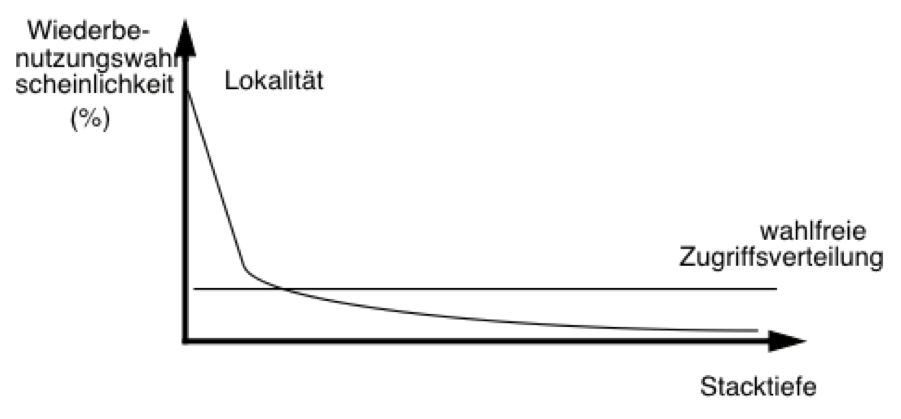
\includegraphics[width = 10cm]{Pictures/Ue07_Aufgabe2_Zusatz2.png}
\end{center}

Ausnahmen in der Monotonie können z.B. durch das Schreiben ins Log oder Warten auf Sperren auftreten.
\end{solution}

%\item Was sind die Grundideen der in der Vorlesung vorgestellten Ersetzungsstrategien? \\Was sind die Vor- und Nachteile dieser einzelnen Strategien?
%
%\begin{note}
%	Evtl Vorstellung mit Skizze: \\
%	FIFO: Stack mit \glqq Ersetzungzeiger\grqq\\
%	LFU: Nach Zugriffen sortierte Liste (Mit Counter)\\
%	LRU: Nach Letztem Zugriffsalter Sortierte Liste (Jeder benutze Block kommt nach ganz oben)\\
%	CLOCK: Uhr anzeichnen mit Benutzt-Bit
%\end{note}
%
%\begin{solution}
%\begin{tabular}{|c|p{6cm}|p{6cm}|}
%	\hline
%	& Welche Blöcke werden verdrängt? &Vor- und Nachteile \\
%	\hline
%	FIFO & Der Block, der am Längsten im Puffer liegt wird verdrängt. & Häufig genutzte Blöcke verschwinden schnell aus dem Puffer. \\
%	\hline
%	LFU & Der Block, der am wenigsten genutzt wurde wird verdrängt. & Einmal häufig genutzte Blöcke verschwinden nie aus dem Puffer. \\
%	\hline
%	LRU & Der Block, der am Längsten nicht genutzt wurde wird verdrängt. & Stapelverwaltung sehr aufwändig. \\
%	\hline
%	CLOCK &   Der Block, auf welchen der Zeiger das nächste mal zeigt und welcher seit dem letzten Zeigerdurchlauf nicht genutzt wurde. & Nicht so gut wie LRU aber deutlich effizienter. \\
%	\hline
%\end{tabular}
%\end{solution}


\end{enumerate}
